\section{Implementation}
Our implementation was done in Matlab code. The structure of the Warm Chorus algorithm is quite modular; figure~\ref{fig:struct}, which details the structure of the algortihm, shows that there are at least six distinct processing blocks.
\begin{figure}[ht]
\centering
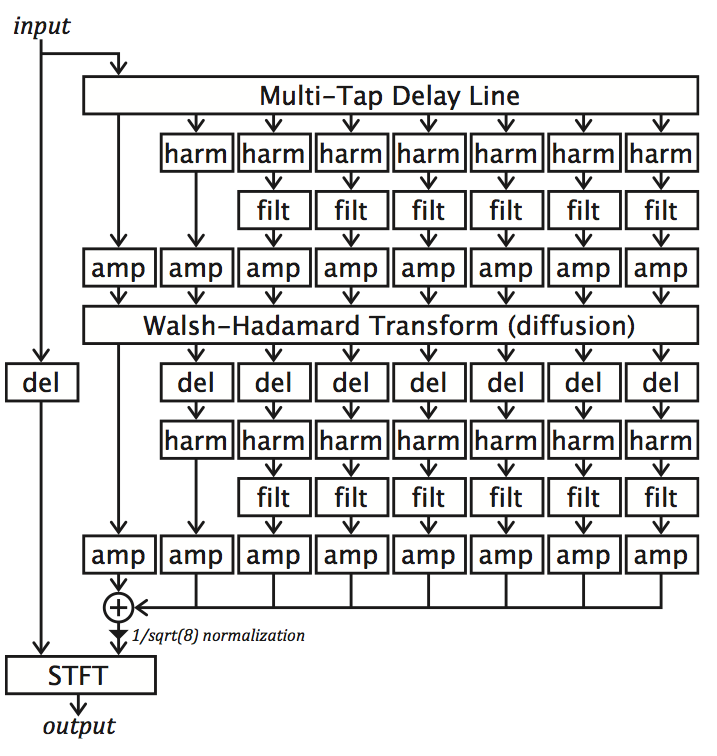
\includegraphics[width= 9cm]{Structure.png}
\caption{Block diagram of the warm chorus algorithm. \cite{dudas}}
\label{fig:struct}
\end{figure}

The flow of the algorithm begins with a multi-tap delay line, which divides the input signal into eight differently delayed paths. The first path is not delayed, as it corresponds to the lead player in the orchestra section. There is also an uneffected path on the left side of the structure, which is only used in the frequency domain processing for some minor corrections.

These eight paths then process the signal with harmonising structures, filters and other common digital signal processing tools. The most important processing block is the harmoniser, which will be explained separately, followed by brief explanations of the other processing blocks. 
